\documentclass{scrbook}
\usepackage{indentfirst}
\usepackage{tikz}
\usepackage{amsmath}
\title{Physics Notes}
\subtitle{A level Physics}
\date{Last Updated \today{}}
\author{Dhruva Lokegaonkar}
\begin{document}
\maketitle

\chapter{Circular Motion, Gravitation and Oscillation}

\section{Circular Motion}

\subsection{Measurement}
	Angles or angular displacement is usually measured in radians. $360^\circ = 2\pi rad$

	\begin{quote}
		One Radian is the angle subtended at the center of a circle by an arc of length equal to the radius of the circle
	\end{quote}

	The time period of rotation is $T$ and frequency is $f$

	\[ \omega = \frac{2\pi}{T} = 2\pi f \]

\subsection{Angular Velocity and Centripetal Force}

	The speed at which a object rotates is called it's angular velocity. It is measured in $rad\ s^{-1}$ and is represented by $\omega$. This is different from it's linear velocity.
	
	\begin{align*}
	\omega = \frac{\Delta \theta}{\Delta t} & & v = \omega r
	\end{align*}

	Even if a rotating object has constant angular velocity, it's linear velocity is not constant. This is because velocity is a vector and an object in circular motion is constantly changing direction. Since there is a change in velocity, there is acceleration. This acceleration is called centripetal acceleration. It can be calculated using a vector diagram.
	
	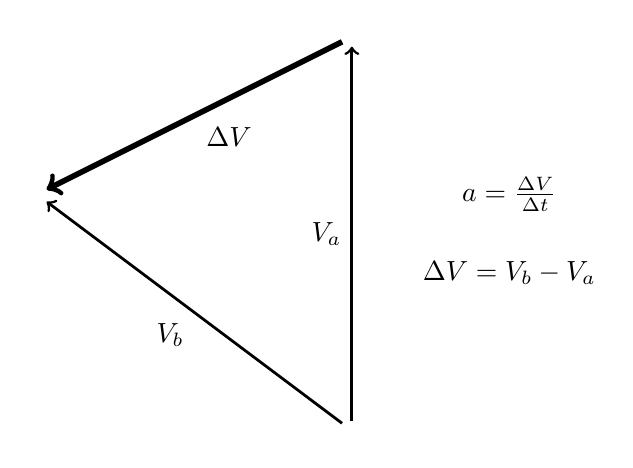
\begin{tikzpicture}[node distance=25mm]
		\node (a) at (0, 0) {};
		\node (b) at (0, 5) {};
		\node (c) at (-4, 3) {};

		\node (eqn) at (2, 3) {};
		\draw (eqn) node {$a = \frac{\Delta V}{\Delta t}$};

		\node (delv) at (2, 2) {};
		\draw (delv) node {$\Delta V = V_b - V_a$};

		\draw[->, line width=1pt] (a) to node[auto] {$V_a$} (b);
		\draw[->, line width=1pt] (a) to node[auto] {$V_b$} (c);
		\draw[->, line width=2pt] (b) to node[auto] {$\Delta V$} (c);
	\end{tikzpicture} 

	The Centripetal acceleration is due to centrepetal forces, which can be gravity or tension in a string. This can be calculated by $F = ma$. Centrepetal acceleration can also be calculated by the follwing formulas: $a = v\omega$, $a = \frac{v^2}{r}$, and $a = \omega ^2 r$. Multiplying by mass gives $F = mv\omega$, $F = \frac{mv^2}{\omega}$, and $F = m\omega^2r$

\section{Gravitation}

\subsection{Newton's Law of Gravitation}

	\begin{quote}
		Any two point masses attract each other with a force that is directly proportional to the product of their masses and inversely proportional to the square of the seperation.
	\end{quote}

	Newtons law can be summaried in the folling equations.
	
	\begin{align*}
		\text{force} &\propto \text{product  of  masses} &
		\\
		\text{force} &\propto \frac{1}{\text{distance}^2} &
		\\
		F &= \frac{GMm}{r^2} & \text{Introducing the constant G, where } G = 6.67\times 10^{-11} Nm^2kg^{-2}
	\end{align*}

\subsection{Gravitational Field Strength}

	\begin{quote}
		The gravitational field strength at a point is the gravitational force exerted per unit mass on a object at a poiny
	\end{quote}

	This is represented by $g$

	\begin{align*}g = \frac{F}{m} & & g = \frac{GM}{r^2}\end{align*}
	
\subsection{Gravitational Potential}

	\begin{quote}
		The gravitational potential at a point is the work done per unit mass to bring a abject from inifinty to a point
	\end{quote}

	It is zero at infinity and negative at any point in the universe. It is represented by the greek letter $\phi$ (phi) and is calculated using the following formula

	\[ \phi = \frac{-GM}{r} \]

\subsection{Orbiting Under Gravity}

	The equations of circular motion and gravitation can be combined to give the equation for orbits under gravity

	\[ F = \frac{mv^2}{r} = \frac{GMm}{r^2}\]
	\[ \text{so } v^2 = \frac{GM}{r}\]

	For an object in a geostationary orbit, the time period can be calculated by using the folling formula

	\[ T^2 = \left(\frac{4\pi^2}{GM}\right)r^3 \]

\section{Oscillations}

	Oscillations or vibrations are to and fro motions. They have three key properties: Frequency, amplitude and period

\subsection{Phase}

	Phase describes the point that an oscillating mass has reached within the complete cycle of an oscillation. It is often measured in degrees or radians. 

\subsection{Simple Harmonic Motion (s.h.m.)}

	There are three requirements for a mechanical system to be in s.h.m:

	\begin{itemize}
		\item
			A mass that oscillates
		\item
			A position where the mass is in equilibrium 
		\item
			A restoring force that acts to return the mass to it's equilibrium position.
	\end{itemize}

	The force is directly proportional to the displacement from the equilibrium position. The following equations describe s.h.m for a oscillator which is at the equilibrium position at $t = 0$

	\begin{align*}
		x &= x_0\sin{\omega t}
		\\
		v &= v_0\cos{\omega t}
		\\
		a &= -\omega^2x
		\\
		v &= \pm \omega \sqrt{x_0^2 - x^2}
		\\
		v_{max} &= \omega x_0
	\end{align*}

\subsection{Resonance and Damping}

	Resonance is a phenomenon observed in systems with forced oscillations. The following statements apply to systems in resonance

	\begin{itemize}
		\item
			It's natural frequency is equal to the frequency of the driver.
		\item
			It's amplitude is maximum
		\item
			It absorbs the greatest possible energy from the driver.
	\end{itemize}

	Damping is when a oscillating system loses energy (due to friction or air resistance). Critical Damping is minimum amount of energy required to return a damped system to equilibrium without oscillating

\end{document}
